\chapter{星系的性质}
\section{星系分类}
目前最广泛使用的星系分类是\textbf{哈勃序列}。哈勃根据星系的整体形态,将它们分成三个大类:\textbf{椭圆星系、漩涡星系和不规则星系}。其中漩涡星系又根据是否带棒分为\textbf{正常漩涡星系}和\textbf{棒旋星系};椭圆星系和漩涡星系之间还存在一类\textbf{透镜状星系}。通过哈勃序列可以确定一个星系的哈勃类型,见图\ref{fig:hubblesequence}。

\begin{figure}[hbt]
  \centering
  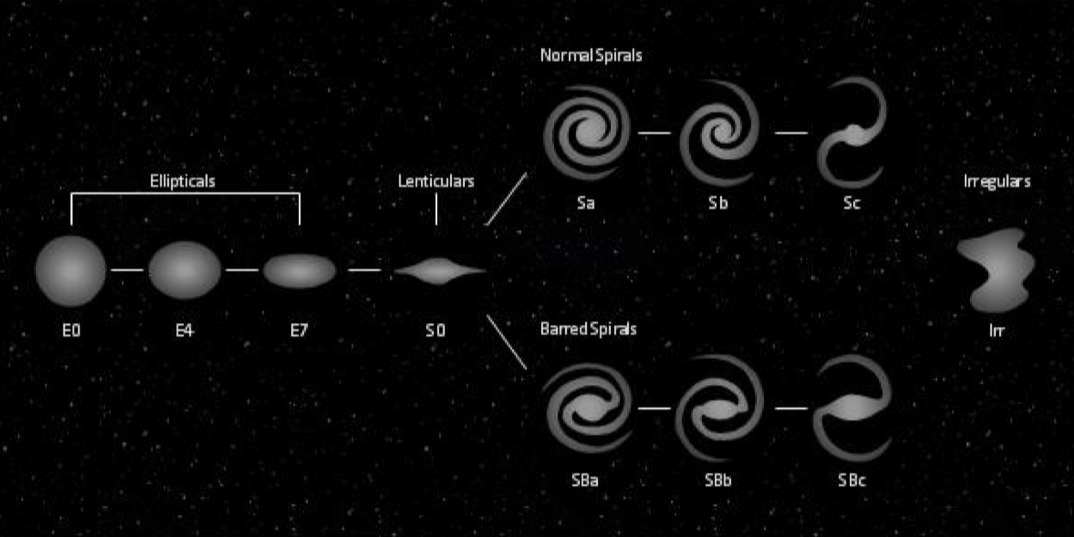
\includegraphics[width=12cm]{chapters/25/fork}
  \caption{星系类型的哈勃音叉形图}
  \label{fig:hubblesequence}
\end{figure}

\section{漩涡星系和不规则星系}
前面提到,可以用21\,cm线来探测气体的分布,因为计算表明其光深约等于中性氢的柱密度。由于它位于微波波段,不容易被星际介质散射,同时也能穿过地球大气,因此也是探测星系结构的很好工具。而通过21\,cm线的多普勒频移,我们还可以探测星系的运动情况。

\subsection{等照度线}
描绘相同面亮度的轮廓被称为\textbf{等照度线},天文学家一直希望通过定义某个等照度线作为星系的半径。对于银河系,一种常用的定义方式是规定具有面亮度$\mu_H=26.5\;B-\mathrm{mag\;arcsec^{-2}}$等照度线的椭球的投影半长轴为半径,这被称为\textbf{霍姆伯格半径(Holmberg radius)}$r_H$。还有一种常用半径是\textbf{有效半径}$r_e$,其定义是包含了星系一半光度的投影半径。

在有效半径$r_e$处的面亮度$\mu_e$的大小,与星系的面亮度随半径的分布有关,而这个分布为\textbf{Sérsic profile}
\begin{equation}
  \mu(r)=\mu_e+8.3268\left[\left({r\over r_e}\right)^{1/n}-1\right]
\end{equation}

它是银核的$r^{1/4}$ de Vaucouleurs profile的推广形式,其中$n, \mu_e, \r_e$是用于与实际面亮度拟合的自由参数。

\subsection{塔利-费希尔关系}
星系的气体受引力束缚转动,因此最大转动速度和中心质量存在一定关系,由于暗物质晕的存在且质量远大于星系质量,因此最大转动速度可以近似为常数,而对于所有漩涡星系,存在相同的质光比$M/L\equiv 1/C_\mathrm{ML}$,以及假设相同的面亮度$L/R^2\equiv C_\mathrm{SB}$,我们可以得到星系光度和最大转动速度的关系:
\begin{equation}
  L={C_\mathrm{ML}^2\over C_\mathrm{SB}}{V_\mathrm{max}^4\over G^2}=CV_\mathrm{max}^4
\end{equation}

根据光度和星等的关系,可以将上式写为:
\begin{equation}
  M=-10\log_{10}V_\mathrm{max}+\mathrm{constant.}
\end{equation}

这种星系光度和最大旋转速度的关系最早在1977年被Tully和Fisher在观测上发现,也因此被命名为\textbf{塔利-费希尔关系}。

\subsection{超大质量黑洞}
通过对银河系中心处恒星的运动表明,银河系中心存在超大质量黑洞Sgr A*。对于其质量的测量,可以通过恒星运动轨迹来测定,但是还有一种方法是通过速度弥散来得到其维里质量。

前面说过引力束缚的平衡系统满足维里定理,即动能和引力势能存在确定关系,动能对应的就是速度,而观测上我们往往只能探测到速度的径向分量,并定义相关的速度弥散,因此我们可以通过速度弥散和维里定理来定义\textbf{维里质量}:
\begin{equation}
  M_\mathrm{virial}\approx{5R\sigma_r^2\over G}
\end{equation}

\subsection{漩涡结构}
关于漩涡星系的漩涡结构是如何形成的,有多种模型来解释,但是其中比较合理和广泛接受的是\textbf{密度波理论}。

这种理论认为漩涡星系的旋臂是气体压缩和恒星形成的波,在银盘中运动。气体从后面进入旋臂,被压缩,形成恒星。旋臂的形式由尘埃带、高气体密度区和新形成的OB恒星描绘。

更具体的解释是,如图\ref{fig:densitywave},由于不同半径的恒星的公转轨道并不是同轴的椭圆,而是存在一个相位差,相位差会导致旋转过程中恒星的密度分布会不同,从而形成了旋臂。

\begin{figure}[hbt]
  \centering
  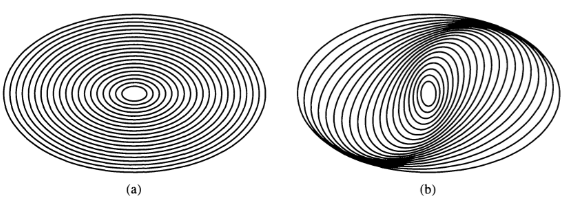
\includegraphics[width=10cm]{chapters/25/densitywave}
  \caption{密度波形成示意图。(a)正常同轴的恒星绕转椭圆轨道(b)彼此有一定夹角的恒星绕转椭圆轨道,可以形成双旋臂}
  \label{fig:densitywave}
\end{figure}

实际漩涡星系内的恒星当然不可能都具有如此理想的椭圆轨道,但却同样会形成这样的密度波旋臂。

\section{椭圆星系}
不像漩涡星系的气体有较统一的转动方向,对于椭圆星系来说,气体的速度弥散更高,因此无法具有漩涡星系那样的光度和最大旋转速度的关系。但是通过维里定理和一些简单假设,也可以得到椭圆星系光度和中心速度弥散的关系——\textbf{费伯-杰克逊关系}:
\begin{equation}
  L\propto\sigma_0^4
\end{equation}
